%%%%%%%%%%%%%%%%%%%%%%%%%%%%%%%%%%%%%%%%%
% Lachaise Assignment
% LaTeX Template
% Version 1.0 (26/6/2018)
%
% This template originates from:
% http://www.LaTeXTemplates.com
%
% Authors:
% Marion Lachaise & François Févotte
% Vel (vel@LaTeXTemplates.com)
%
% License:
% CC BY-NC-SA 3.0 (http://creativecommons.org/licenses/by-nc-sa/3.0/)
%
%%%%%%%%%%%%%%%%%%%%%%%%%%%%%%%%%%%%%%%%%

%----------------------------------------------------------------------------------------
%	PACKAGES AND OTHER DOCUMENT CONFIGURATIONS
%----------------------------------------------------------------------------------------

\documentclass{article}

%%%%%%%%%%%%%%%%%%%%%%%%%%%%%%%%%%%%%%%%%
% Lachaise Assignment
% Structure Specification File
% Version 1.0 (26/6/2018)
%
% This template originates from:
% http://www.LaTeXTemplates.com
%
% Authors:
% Marion Lachaise & François Févotte
% Vel (vel@LaTeXTemplates.com)
%
% License:
% CC BY-NC-SA 3.0 (http://creativecommons.org/licenses/by-nc-sa/3.0/)
%
%%%%%%%%%%%%%%%%%%%%%%%%%%%%%%%%%%%%%%%%%

%----------------------------------------------------------------------------------------
%	PACKAGES AND OTHER DOCUMENT CONFIGURATIONS
%----------------------------------------------------------------------------------------

\usepackage{amsmath,amsfonts,stmaryrd,amssymb} % Math packages

\usepackage{enumerate} % Custom item numbers for enumerations

\usepackage[ruled]{algorithm2e} % Algorithms

\usepackage[framemethod=tikz]{mdframed} % Allows defining custom boxed/framed environments

\usepackage{listings} % File listings, with syntax highlighting

\usepackage{color} %red, green, blue, yellow, cyan, magenta, black, white
\definecolor{mygreen}{RGB}{28,172,0} % color values Red, Green, Blue
\definecolor{mylilas}{RGB}{170,55,241}
\usepackage{float}
\usepackage{amsmath}% http://ctan.org/pkg/amsmath
\newcommand\Inn{%
  \mathrel{\ooalign{$\subset$\cr\hfil\scalebox{0.8}[1]{$=$}\hfil\cr}}%
}
% \mathcode`*=\string"8000

\lstset{
	basicstyle=\ttfamily, % Typeset listings in monospace font
}


% matlab desciption
% usage \lstinputlisting{/path/to/matlab/code.m}

\lstset{language=Matlab,%
    %basicstyle=\color{red},
    breaklines=true,%
    morekeywords={matlab2tikz},
    keywordstyle=\color{blue},%
    morekeywords=[2]{1}, keywordstyle=[2]{\color{black}},
    identifierstyle=\color{black},%
    stringstyle=\color{mylilas},
    commentstyle=\color{mygreen},%
    showstringspaces=false,%without this there will be a symbol in the places where there is a space
    numbers=none,%
    numberstyle={\tiny \color{black}},% size of the numbers
    numbersep=9pt, % this defines how far the numbers are from the text
    emph=[1]{for,end,break},emphstyle=[1]\color{red}, %some words to emphasise
    %emph=[2]{word1,word2}, emphstyle=[2]{style},
}


%----------------------------------------------------------------------------------------
%	DOCUMENT MARGINS
%----------------------------------------------------------------------------------------

\usepackage{geometry} % Required for adjusting page dimensions and margins

\geometry{
	paper=a4paper, % Paper size, change to letterpaper for US letter size
	top=2.5cm, % Top margin
	bottom=3cm, % Bottom margin
	left=2.5cm, % Left margin
	right=2.5cm, % Right margin
	headheight=14pt, % Header height
	footskip=1.5cm, % Space from the bottom margin to the baseline of the footer
	headsep=1.2cm, % Space from the top margin to the baseline of the header
	%showframe, % Uncomment to show how the type block is set on the page
}

%----------------------------------------------------------------------------------------
%	FONTS
%----------------------------------------------------------------------------------------

\usepackage[utf8]{inputenc} % Required for inputting international characters
\usepackage[T1]{fontenc} % Output font encoding for international characters

\usepackage{XCharter} % Use the XCharter fonts

%----------------------------------------------------------------------------------------
%	COMMAND LINE ENVIRONMENT
%----------------------------------------------------------------------------------------

% Usage:
% \begin{commandline}
%	\begin{verbatim}
%		$ ls
%
%		Applications	Desktop	...
%	\end{verbatim}
% \end{commandline}

\mdfdefinestyle{commandline}{
	leftmargin=10pt,
	rightmargin=10pt,
	innerleftmargin=15pt,
	middlelinecolor=black!50!white,
	middlelinewidth=2pt,
	frametitlerule=false,
	backgroundcolor=black!5!white,
	frametitle={Command Line},
	frametitlefont={\normalfont\sffamily\color{white}\hspace{-1em}},
	frametitlebackgroundcolor=black!50!white,
	nobreak,
}

% Define a custom environment for command-line snapshots
\newenvironment{commandline}{
	\medskip
	\begin{mdframed}[style=commandline]
}{
	\end{mdframed}
	\medskip
}

%----------------------------------------------------------------------------------------
%	FILE CONTENTS ENVIRONMENT
%----------------------------------------------------------------------------------------

% Usage:
% \begin{file}[optional filename, defaults to "File"]
%	File contents, for example, with a listings environment
% \end{file}

\mdfdefinestyle{file}{
	innertopmargin=1.6\baselineskip,
	innerbottommargin=0.8\baselineskip,
	topline=false, bottomline=false,
	leftline=false, rightline=false,
	leftmargin=2cm,
	rightmargin=2cm,
	singleextra={%
		\draw[fill=black!10!white](P)++(0,-1.2em)rectangle(P-|O);
		\node[anchor=north west]
		at(P-|O){\ttfamily\mdfilename};
		%
		\def\l{3em}
		\draw(O-|P)++(-\l,0)--++(\l,\l)--(P)--(P-|O)--(O)--cycle;
		\draw(O-|P)++(-\l,0)--++(0,\l)--++(\l,0);
	},
	nobreak,
}

% Define a custom environment for file contents
\newenvironment{file}[1][File]{ % Set the default filename to "File"
	\medskip
	\newcommand{\mdfilename}{#1}
	\begin{mdframed}[style=file]
}{
	\end{mdframed}
	\medskip
}

%----------------------------------------------------------------------------------------
%	NUMBERED QUESTIONS ENVIRONMENT
%----------------------------------------------------------------------------------------

% Usage:
% \begin{question}[optional title]
%	Question contents
% \end{question}

\mdfdefinestyle{question}{
	innertopmargin=1.2\baselineskip,
	innerbottommargin=0.8\baselineskip,
	roundcorner=5pt,
	nobreak,
	singleextra={%
		\draw(P-|O)node[xshift=1em,anchor=west,fill=white,draw,rounded corners=5pt]{%
		Question \theQuestion\questionTitle};
	},
}

\newcounter{Question} % Stores the current question number that gets iterated with each new question

% Define a custom environment for numbered questions
\newenvironment{question}[1][\unskip]{
	\bigskip
	\stepcounter{Question}
	\newcommand{\questionTitle}{~#1}
	\begin{mdframed}[style=question]
}{
	\end{mdframed}
	\medskip
}

%----------------------------------------------------------------------------------------
%	WARNING TEXT ENVIRONMENT
%----------------------------------------------------------------------------------------

% Usage:
% \begin{warn}[optional title, defaults to "Warning:"]
%	Contents
% \end{warn}

\mdfdefinestyle{warning}{
	topline=false, bottomline=false,
	leftline=false, rightline=false,
	nobreak,
	singleextra={%
		\draw(P-|O)++(-0.5em,0)node(tmp1){};
		\draw(P-|O)++(0.5em,0)node(tmp2){};
		\fill[black,rotate around={45:(P-|O)}](tmp1)rectangle(tmp2);
		\node at(P-|O){\color{white}\scriptsize\bf !};
		\draw[very thick](P-|O)++(0,-1em)--(O);%--(O-|P);
	}
}

% Define a custom environment for warning text
\newenvironment{warn}[1][Warning:]{ % Set the default warning to "Warning:"
	\medskip
	\begin{mdframed}[style=warning]
		\noindent{\textbf{#1}}
}{
	\end{mdframed}
}

%----------------------------------------------------------------------------------------
%	INFORMATION ENVIRONMENT
%----------------------------------------------------------------------------------------

% Usage:
% \begin{info}[optional title, defaults to "Info:"]
% 	contents
% 	\end{info}

\mdfdefinestyle{info}{%
	topline=false, bottomline=false,
	leftline=false, rightline=false,
	nobreak,
	singleextra={%
		\fill[black](P-|O)circle[radius=0.4em];
		\node at(P-|O){\color{white}\scriptsize\bf i};
		\draw[very thick](P-|O)++(0,-0.8em)--(O);%--(O-|P);
	}
}

% Define a custom environment for information
\newenvironment{info}[1][Info:]{ % Set the default title to "Info:"
	\medskip
	\begin{mdframed}[style=info]
		\noindent{\textbf{#1}}
}{
	\end{mdframed}
}
 % Include the file specifying the document structure and custom commands
\usepackage{graphicx}
\newcommand{\ts}{\textsuperscript}
\usepackage{float}


%----------------------------------------------------------------------------------------
%	ASSIGNMENT INFORMATION
%----------------------------------------------------------------------------------------

\title{Computational Engineering - Engr 8103 \\ Problem Set \#8} % Title of the assignment

\author{Allen Spain\\ \texttt{avs81684@uga.edu}} % Author name and email address

\date{University of Georgia --- 26 November 2019 } % University, school and/or department name(s) and a date

%----------------------------------------------------------------------------------------

\begin{document}

\maketitle % Print the title

%----------------------------------------------------------------------------------------
%	INTRODUCTION
%----------------------------------------------------------------------------------------

\section*{Problem 1} % Unnumbered section
(10 pts.) Consider the following transport PDE

\begin{align*}
u_{t} = D_{u_{xx}} - Fu_{x} \\
u(0,x) = \frac{2x}{1+x^{4}} \quad 0 \leq x \leq 20 \\
u(t,0) = 0 \quad 0 \leq t \leq 3 \\
u(t,20) = 0 \quad 0 \leq t \leq 3
\end{align*}

\noindent
Where $u(t, x)$ represents the drug concentration at time t seconds and x inches away from a reference point on the vein, located slightly behind the point of injection. $u(0, x)$ represents the initial drug concentration through the blood vein a moment after the injection:


Discretize this PDE using backward time for ut, backward space for ux and the regular second derivative method for uxx, the same one we used in class for the diffusion equation. Assuming $D=0.5$,$F=2$,$dt=2$ and $dx=4$,write down the matrix $M$ where:

\begin{align*}
M\begin{bmatrix}u^{n+1}_{2}\\u^{n+1}_{3}\\u^{n+1}_{4}\\u^{n+1}_{5}\end{bmatrix} = b
\end{align*}

Discretizing using $B_{t}B_{x}$
\begin{align*}
u_{t} = u^{n}_{k} - u^{n-1}_{k}
u_{x} = u^{k}_{n} - u^{n}_{k-1}
u_{xx} = u^{n}_{k-1} - 2u^{n}_{k} + u^{n}_{k+1}
\end{align*}
Given that

\begin{align*}
u_{t} = Du_{xx} - Fu_{x}
\end{align*}
The aforementioned discretization $u_{t}$ yields:

\begin{align*}
	u_{t} = \frac{u^{n}_{k} - u^{n-1}_{k}}{dt} \\
	u^{n}_{k} - u^{n-1}_{k} = \frac{D dt}{(dx)^{2}} [u^{n}_{k-1} - 2u^{n}_{k} + u^{n}_{k+1}] - \frac{F dt}{dx}[u^{n}_{k} - u^{n}_{k-1}]
\end{align*}

Define: $L_{1} = \frac{Ddt}{(dx)^{2}}$ and $L_{2} = \frac{Fdt}{dx}$

\begin{align*}
\therefore  u^{n-1}_{k} = - (L_{1} + L_{2})u^{n+1}_{k-1} + (2L_{1} - L_{2} + 1)u^{n}_{k} - L_{1}u^{n}_{k+1}
\end{align*}

\begin{align*}
\text{Assume: } n \rightarrow n + 1 \\
L_{1} = 0.5(\frac{1}{2}) = \frac{1}{4} \\
L_{2} = 2(\frac{1}{2}) = 1 \\
u^{n}_{k} = - (L_{1} + L_{2})u^{n+1}_{k-1} + (2L_{1} - L_{2} + 1)u^{n}_{k} - L_{1}u^{n}_{k+1}
\end{align*}

So the matrix M can be defined as:
\begin{align*}
\begin{bmatrix} (L_{2} + L_{2} - 1) && -L_{1} && 0 && 0\\ -(L_{1} + L_{2}) && (L_{2} + L_{2} - 1) && -L_{1} && 0\\ 0 &&  -(L_{1}+ L_{2}) && (2L_{1} + L_{2} + -1) && -L_{1} \\0 && 0 && -(L_{1} + L_{2}) && (L_{2} + L_{2} - 1) \end{bmatrix}
\end{align*}

(b) (10 pts.) Write a Matlab code to solve this PDE using the discretization you developed in part (a). Use $D = 0.5$, $F = 2$, $dt = 0.02$, $dx = 0.02$. Note that since backward time methods tend to be more stable, you can afford to use a finer mesh for the space dimension (smaller dx values.) Your code should plot the initial drug concentration and the drug concentrations after one, two and three seconds on the same figure. In other words, plot $u(0, x)$, $u(1, x)$, $u(2, x)$ and $u(3, x)$ vs x. Identify each plot using a legend. Include a hard copy of this figure with your HW solutions.

(b)
\lstinputlisting{/Users/allenspain/Documents/hw8/drug_Bt.m}
Had some errors coding despite the math seeming correct

\begin{figure}[H]
  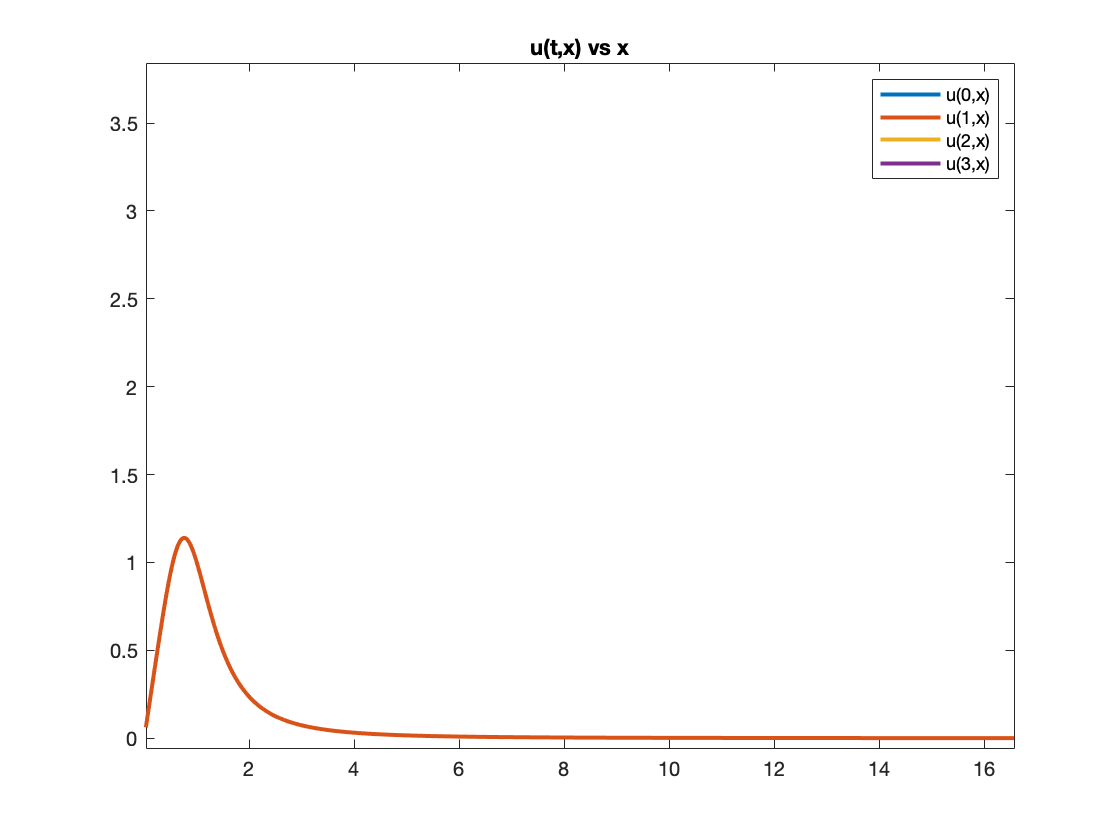
\includegraphics[width=\linewidth]{docs/1b.png}
  \caption{1b}
  % \label{fig:boat1}
\end{figure}

(c) (5 pts.) Now assume faster blood flow; that is $F = 6$. Repeat part (b) for this case. Does the figure look realistic? Why not? Explain.
- The concetration would have an abnormal retractio rate, and would therefore diminish faster then realistic.

\section*{Problem 2} % Unnumbered section
(10 pts.) Consider the same PDE where one of the boundary conditions is changed from Dirichlet to Neumann:

\begin{align*}
M\begin{bmatrix}u^{n+1}_{2}\\u^{n+1}_{3}\\u^{n+1}_{4}\\u^{n+1}_{5}\\u^{n+1}_{6}\end{bmatrix} = b
\end{align*}


(a)
\begin{align*}
\begin{bmatrix} (L_{2} + L_{2} - 1) && -L_{1} && 0 && 0\\ -(L_{1} + L_{2}) && (L_{2} + L_{2} - 1) && -L_{1} && 0\\ 0 &&  -(L_{1}+ L_{2}) && (2L_{1} + L_{2} + -1) && -L_{1} \\0 && 0 && -(L_{1} + L_{2}) && (L_{2} + L_{2} - 1) \\0 && 0 && 0 &&-(L_{1} + L_{2})\end{bmatrix}
\end{align*}

(b)
\lstinputlisting{/Users/allenspain/Documents/hw8/drug_Bt_Nbc.m}
Had some errors coding despite the math seeming correct

\end{document}
